\documentclass[10pt]{article}
\usepackage{fullpage}
\usepackage{graphicx}
\usepackage{amssymb}
\newcommand{\tab}{\hspace*{2em}}
\begin{document}
	\begin{flushright}
	Lindsey Bieda and Joe Frambach\\
	Greedy Algorithm and Dynamic Programming Problems\\
	9.15.2011
	\end{flushright}
	\noindent
	15. You have $n$ heterosexual men and $n$ heterosexual women.  Each man ranks the women in order of
			preference.   Each woman ranks the men in order of preference.   Consider the following incredibly
			stereotypical courting algorithm. On stage $i$, each man goes to pitch woo on the porch of the woman
			that he prefers most among all women that have not rejected him yet.  At the end of the stage the
			woman rejects all the men on her porch but the one that she favors most.  Note that a women may
			not reject a man in some stage, but later end up rejecting that man if a better prospect arrives on her
			porch. If it should ever happen that there is exactly one man on each porch, the algorithm terminates,
			and each woman marries the man on her porch. (You may be interested to know that medical schools
			really use this algorithm to fill intern positions.)
			\begin{enumerate}
				\item[(a)]  Give an upper bound as a function of $n$ of the number of stages in this algorithm.\\
										% answer here
										\\
										\\
										The worst case occurs when all men have identical preferences. They ``follow" each other
										from porch to porch, dropping one man each stage. Worst-case stages for $n$ men is $n$.\\
				\item[(b)]  A marriage assignment is stable if there does not exist a man $x$ and a woman $y$  such that $x$
										prefers $y$ to his assigned mate, and $y$ prefers $x$ to her assigned mate. Clearly adultery is a risk if
										a marriage assignment is not stable. Prove that this algorithm leads to a stable marriage.\\
										% answer here
										\\
										\\
										Assume that the above algorithm creates the following parings: $M_x, W_y$ and $M_i, W_j$ - where $M_x, M_i$ are
										a part of a set of men and $W_y, W_j$ are a part of a set of women. Assume that in this set $M_x, W_j$ prefer
										each other and $M_i, W_y$ prefer each other.\\
										$W_j \leftrightarrow M_x \dashleftarrow \dashrightarrow W_y \leftrightarrow M_i$, dashed arrow is a mutual 
										preference and solid is a marriage. For this to be the case some stage S (fig. 1) must occur.\\
										\begin{figure}[h]
											\centering
												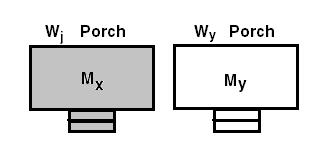
\includegraphics{15b.png}
											  \caption{stage S.}
										\end{figure}
										\linebreak
										However, $M_x$ should have gone to $W_y$'s porch and $M_i$ should have gone to $W_j$'s porch because of higher
										preference. 
				\item[(c)]  A stable marriage $M$ is man optimal if for every man $x$, $M$ is the best possible stable marriage.
										That is, in every stable marriage other than $M$, $x$ ends up with a woman no more preferable to
										him than the woman he is married to in $M$.  Prove or disprove the above algorithm produces a
										man optimal stable marriage.
										% answer here
				\item[(d)]  A stable marriage $M$  is woman optimal if for every woman $y$,  $M$  is the best  possible stable
										marriage.   That is,  in every  stable marriage other  than $M$,  $y$  ends  up with a  man no  more
										preferable to her than the man she is married to in $M$.  Prove or disprove the above algorithm
										produces a woman optimal stable marriage.
										% answer here
				\item[(e)]  A stable marriage $M$ is man pessimal if for every man $x$, $M$ is the worst possible stable marriage.
										That is, in every stable marriage other than $M$, $x$ ends up with a woman no less preferable to her
										that the woman he is married to in $M$.  Prove or disprove the above algorithm produces a man
										pessimal stable marriage.
										% answer here
				\item[(f)]  A stable marriage $M$  is woman pessimal if for every woman $y$, $M$  is the worst possible stable
										marriage. That is, in every stable marriage other than $M$, $y$ ends up with a man no less preferable
										to her list than the man she is married to in $M$. Prove or disprove the above algorithm produces
										a woman pessimal stable marriage.
										% answer here
			\end{enumerate}
	\\
	\\
	1. Consider the recurrence relation $T(0) = T(1) = 2$ and for $n > 1$
	
	\[T(n) = \sum\limits_{i=1}^{n-1} T(i)T(i-1) \]
	
	\noindent
	We consider the problem of computing $T(n)$ from $n$.
	\begin{enumerate}
		\item[(a)] 	Show that if you implement this recursion directly in say the C programming language, that the
								program would use exponentially, in $n$, many arithmetic operations.
								% answer here
										\begin{figure}[h]
											\centering
												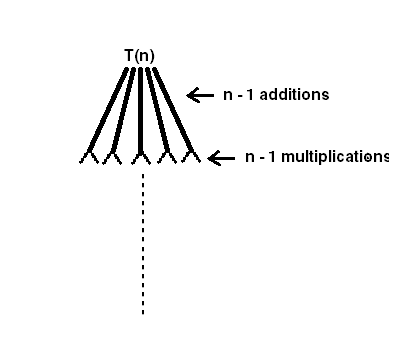
\includegraphics{1a.png}
											  \caption{Part of the call tree.}
										\end{figure}
										The above call tree will have a depth of $n$, each node requires $O(n)$ function calls and 
										each function call requires $O(n^2)$ arithmetic operations (see answer b).\\
										Therefore, the number of arithmetic operations is $O(n^4)$.\\
										\\
		\item[(b)] 	Explain how, by not recomputing the same $T(i)$ value twice, one can obtain an algorithm for this
								problem that only uses $O(n^2)$ arithmetic operations.
								% answer here
										\\
										\\
										\begin{array}{cccc}
											function~call & additions & multiplications & function~calls\\
											T(n) & n-1 & n-1 & 2(n-1)\\
											T(n-1) & n-2 & n-2 & 2(n-2)\\
											\vdots \\
											T(2) & 1 & 1 & 2\\
											T(1) & 0 & 0 & 0\\
											T(0) & 0 & 0 & 0
										\end{array}
										\\
										T(n) requires $\frac{(n-1)^2 - (n-2)}{2} + \frac{(n-1)^2 - (n-2)}{2} = (n-1)^2 - (n-2) = 0(n^2)$
		\item[(c)]	Give an algorithm for this problem that only uses $O(n)$ arithmetic operations.
								% answer here
								\begin{verbatim}
									T[]
									T[0] = 2
									T[1] = 2
									
									For i = 2 to n
									    T[i] = T[i-1]*(1 + T[i-2])								
								\end{verbatim}
								\\
								Requires $n$ iterations and is therefore $O(n)$.
	\end{enumerate}
\end{document}